% ============================================================
% file: nn_dag.tex
% Simple computational DAG for one neuron / operation chain
% ============================================================

\documentclass{standalone}
\usepackage{tikz}
\usetikzlibrary{arrows.meta, positioning, calc}
\usepackage{amsmath}
\usepackage{amssymb}

\begin{document}

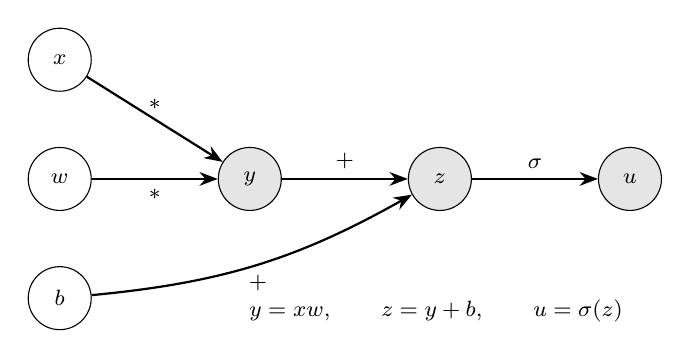
\begin{tikzpicture}[
  node/.style={
    circle,
    draw,
    minimum width=0.8cm,
    minimum height=0.8cm,
    align=center,
    fill=gray!20
  },
  leaf/.style={
    node,
    fill=white!20
  },
  every node/.style={font=\footnotesize},
  arrow/.style={-Stealth, thick}
]

% ------------------------------------------------------------
% Leaf nodes
% ------------------------------------------------------------

\node[leaf] (x) {$x$};
\node[leaf, below=0.7cm of x] (w) {$w$};
\node[leaf, below=0.7cm of w] (b) {$b$};

% ------------------------------------------------------------
% Intermediate and output nodes
% ------------------------------------------------------------

\node[node, right=1.6cm of w] (y) {$y$};
\node[node, right=1.6cm of y] (z) {$z$};
\node[node, right=1.6cm of z] (u) {$u$};

% ------------------------------------------------------------
% Computational dependencies
% ------------------------------------------------------------

\draw[arrow] (x) -- node[above] {$*$} (y);
\draw[arrow] (w) -- node[below] {$*$} (y);

\draw[arrow] (y) -- node[above] {$+$} (z);
\draw[arrow] (b) to[bend right=12] node[below] {$+$} (z);

\draw[arrow] (z) -- node[above] {$\sigma$} (u);

% ------------------------------------------------------------
% Optional equations under the graph
% ------------------------------------------------------------

\node[align=center, below=1.0cm of z] {
$y=xw,\qquad z=y+b,\qquad u=\sigma(z)$
};

\end{tikzpicture}

\end{document}